\ofsubsection{Combate}
%
\ofquote{"Chega de brincadeiras expositivas. É hora de lutarmos como homens. E Damas. E damas que se vestem como homens."}{Gilgamesh}\\
%
\includegraphics[width=\columnwidth]{./art/images/ff13-2.jpg}
%
\vfill
%
Encontros de \accf{Combate} são uma série de Rodadas (\accf{r}) e durante cada uma delas, cada combatente tem um turno.
No início de cada combate, ambos os grupos escolhem quem agirá no primeiro turno de cada rodada e o MJ decide quem dos inimigos vai primeiro.
Assim, as partes opostas se alternam até que cada combatente tenha agido e a rodada termina. 
A ordem de turno para cada lado é decidido da seguinte maneira: ao final de seu turno, cada combatente escolhe um aliado que ainda não agiu nessa rodada para agir no próximo turno do seu grupo. 
Se um dos lados tem mais combatentes, eles podem agir em turnos consecutivos ao final de cada rodada até que cada participante tenha agido. 
Anuncie o começo e o fim de cada rodada para evitar confusão. Quando um grupo emboscar o outro antes do combate, o MJ pode decidir que eles ganham uma \accf{Rodada Surpresa}. 
Nesse caso, o grupo que surpreendeu age antes mesmo do combate iniciar.
%
\vfill
%
As proficiências em Combate são determinadas por 7 \accf{atributos}. 
Sempre que um cálculo resultar em um valor não inteiro, o resultado é arredondado para baixo.
%
\ofgap
%
\ofmbox{\oficonhp\accf{Pontos de vida (PV)}} aumentam sua durabilidade. Você tem um valor de PV máximo e um atual, se o atual chegar a 0, você cai inconsciente. \ofrow
\ofmbox{\oficonmp\accf{Pontos de Mana (PM)}} são recursos exigidos para o uso de habilidades. Assim com os PV, você tem um valor máximo e um atual. \ofrow
\ofmbox{\oficonstr\accf{Força (FOR)}} aumenta os danos de seus ataques e habilidades físicas. \ofrow
\ofmbox{\oficondef\accf{Defesa (DEF)}} aumenta sua resistência contra danos físicos. \ofrow
\ofmbox{\oficonmag\accf{Magia (MAG)}} aumenta o dano e cura recebidos por suas habilidades mágicas. \ofrow
\ofmbox{\oficonres\accf{Resistência (RES)}} aumenta sua resistência contra danos mágicos. \ofrow
\ofmbox{\oficonagi\accf{Agilidade (AGI)}} permite-o evadir de ataques físicos e determina o quão rápido você se move.
%
\newpage
%
Durante o seu turno você pode se mover uma distância em unidades igual a sua AGI+1 e/ou agir. 
Abaixo está uma lista de \accf{Ações de Combate}, mas o MJ pode permitir que qualquer outras ações possam ser executadas:
%
\vfill
%
\ofmbox{\oficonattack\accf{Ataque:}}
Você ataca um inimigo com sua arma. 
Ele pode se evadir ao superar um \accf{teste de evasão} de DF 12 menos a AGI dele. 
Caso falhe no teste, você reduz o PV dele igual ao dano da sua arma mais sua FOR. 
Se o alvo obter 2, você consegue um \accf{Acerto Crítico}, dobrando seu dano. 
Se ele obter 12, seu ataque erra e o alvo realiza um ataque contra você, que acerta automaticamente. \ofgap
%
\ofmbox{\oficonmagic\accf{Magia:}}
Você usa uma habilidade mágica gastando PM, escolhendo um alvo dentro de seu alcance e concentrando pela duração dela. 
Enquanto estiver concentrando, você não pode agir ou se evadir. 
Após o tempo de conjuração, o efeito da magia afeta o alvo \accf{antes de sua vez} e não pode ser evadido, mesmo se você não estiver mais ao alcance determinado.
Se a magia causar danos ou restaurar PV, adicione sua MAG ao total. 
Cada descrição de magia informa o tempo de conjuração, MP, alvo, alcance e efeito dela. \ofgap
%
\ofmbox{\oficontech\accf{Técnica:}}
Você usa uma habilidade física. 
Técnicas são usadas da mesma maneira que magias, mas o dano e cura delas são amplificados pela sua FOR ao invés de sua MAG, exceto se o uso delas já incluir algum outro bônus, como por exemplo, envolvendo um ataque. \ofgap
%
\ofmbox{\oficondefend\accf{Defender:}}
Todo o dano de ataques recebidos, até o seu próximo turno, é reduzido pela metade. \ofgap
%
\ofmbox{\oficonitem\accf{Item:}}
Você usa um item de seu inventário em si mesmo ou alguém dentro de 1u. \ofgap
%
\ofmbox{\oficonreequip\accf{Re-Equipar:}}
Trocar uma matéria ou peça de equipamento que você está usando por outro que tenha em seu inventário. \ofgap
%
\ofmbox{\oficondash\accf{Correr:}}
Mova-se a um local até sua AGI+1 em unidades.
%
\vfill
%
Combatentes também podem aprender dois tipos de características:\vspace*{0.2cm}\\
\ofmbox{\oficonpassive\accf{Passiva:}} Efeitos que são ativos permanentemente. \ofgap
\ofmbox{\oficonreaction\accf{Reação:}} Permitem a você tomar certas ações no turno de alguma outra pessoa, sob condições específicas.
%
\vfill
%
\ofboxwithtitle{Examplo: Combate}
{
	Squall (4 DEF, 3 AGI, 1 RES) e Seifer (6 FOR, 2 MAG) decidem duelar. 
	Ambos empunham uma Lâmina Pistola (1d Danos) e o MJ decide que Seifer agirá primeiro. 
	Ele começa conjurando Fogaga (6d Dano, 1r Tempo) gastando 12 PM, escolhendo Squall como seu alvo e se concentrando. 
	Squall usa sua vez para Defender. 
	É a vez de Seifer novamente, então Fogaga acontece e Squall sofre \mbox{6d+2-1} de danos. 
	Seifer ainda pode ter sua vez, então ele também ataca. 
	Squall faz um teste de evasão \mbox{DF 12-3}, mas rola [1, 1], ele falha e sofre um Ataque Crítico! 
	Seifer o atinge bem acima de seu nariz com sua lâmina, infligindo \mbox{1d+6-4} de danos (Defender e Ataques Críticos cancelam um ao outro) e deixando uma cicatriz.
}
%
\clearpage
%
\newcommand{\elemicon}[1]{\hspace*{-0.14cm}#1\hspace*{-0.14cm}}
Todo dano causado tem um de dois tipos básicos. 
Exceto se especificado, Ataques e Técnicas são do tipo \accf{Físico}, enquanto Magia e Itens são do tipo \accf{Mágico}. 
Quando você recebe danos físicos, subtraia sua DEF da quantidade e quando receber danos mágicos, de sua RES. 
Adicionalmente, danos podem ter um tipo elemental do qual os combatentes podem ter \accf{fraquezas} ou \accf{resistências}. 
Quando resistente a um tipo de dano, você sofre metade do dano normal e quando fraco, o dobro. 
Resistência e Fraquezas se cancelam entre si e não acumulam. Existem os seguintes tipos elementais: Fogo, Gelo, Raio, Água, Terra, Vento, Sagrado e Escuridão.
%
\vfill
%
\accf{Unidades} (\accf{u}) são a base para se medir distancias, em que 1u é aproximadamente 1m ou 3 pés. 
Personagens normalmente ocupam um círculo de 1u de diâmetro visto por cima. 
Distância de efeitos são descritos pelo seu Alcance e Alvo. 
\accf{Alcance} é a distância máxima entre o centro do conjurador e o centro do efeito. 
Um efeito com alcance de Você é centrado no conjurador e um com alcance Arma, tem a mesma distância da arma usada. 
\accf{Alvo} é a área de efeito com uma distância máxima de seu centro. A menos que indicado o contrário, todos inteiro ou parcialmente na área de efeito são atingidos, incluindo aliados. 
Um efeito com alvo Único, afeta somente um único indivíduo. A seguinte ilustração mostra o uso de um efeito à distância em casos normais e com as duas formas de alvos especiais, Linha e Frontal.
%
\begin{figure}[h!]
		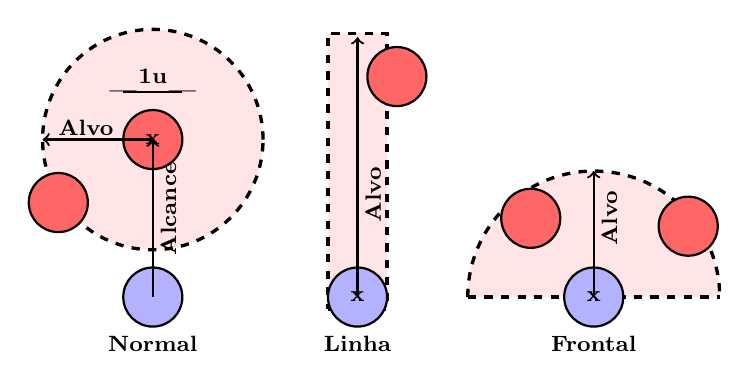
\begin{tikzpicture}[]
		\tikzstyle{test}=[thick, draw, circle, align=center]					
		%Normal
		\node[fill=blue!30!white, test,minimum size = 0.75cm](caster)at (0,0) {};
		\node[](t2)at (0,-0.6) {\bf\footnotesize Normal};
		\node[fill=red!10!white, test, very thick, dashed ,minimum size = 2.8cm](tarea)at (0,2) {};
		\node[fill=red!60!white, test,minimum size = 0.75cm](target)at (0,2) {};
		\node[fill=red!60!white, test,minimum size = 0.75cm](target)at (-1.2,1.2) {};
		\draw[thick, ->](0,0) -- node[] {}(0,2);
		\draw[thick, ->](0,2) -- node[] {}(-1.4, 2);
		\node[rotate=90](t1)at (0.2,1.12) {\bf\footnotesize Alcance};
		\node[](t2)at (-0.85,2.15) {\bf\footnotesize Alvo};
		\node[](t3)at (0,2) {\bf\footnotesize x};
		\node[](fi)at (-0.375,2.6) {\bf\footnotesize |};
		\node[](se)at (0.375,2.6) {\bf\footnotesize |};
		\draw[thick, -](0.375,2.6) -- node[] {}(-0.375,2.6);
		\node[](sca)at (0,2.8) {\bf\footnotesize 1u};		
		%Line
		\node[draw, fill=red!10!white, rectangle, very thick, dashed ,minimum height = 3.5cm, minimum width=0.75cm](tarea)at (2.6,1.6) {};
		\node[fill=blue!30!white, test,minimum size = 0.75cm](caster)at (2.6,0) {};
		\node[](t2)at (2.6,-0.6) {\bf\footnotesize Linha};
		\node[fill=red!60!white, test,minimum size = 0.75cm](target)at (3.1,2.8) {};
		\draw[thick, ->](2.6,0) -- node[] {}(2.6,3.3);
		\node[rotate=90](t1)at (2.8,1.3) {\bf\footnotesize Alvo};
		\node[](t3)at (2.6,0) {\bf\footnotesize x};		
		%Front
		\draw[fill=red!10!white, test, very thick, dashed] (4,0) arc (180:0:1.6cm);
		\draw[dashed, very thick, -](4,0) -- node[] {}(7.2,0);
		\node[fill=blue!30!white, test,minimum size = 0.75cm](caster)at (5.6,0) {};
		\node[](t2)at (5.6,-0.6) {\bf\footnotesize Frontal};
		\draw[thick, ->](5.6,0) -- node[] {}(5.6,1.6);
		\node[rotate=90](t1)at (5.8,1) {\bf\footnotesize Alvo};
		\node[fill=red!60!white, test,minimum size = 0.75cm](target)at (4.8,1) {};
		\node[fill=red!60!white, test,minimum size = 0.75cm](target)at (6.8,0.9) {};
		\node[](t3)at (5.6,0) {\bf\footnotesize x};
		\end{tikzpicture}
\end{figure}
%
\vfill
%
\accf{Campos} são efeitos que ocupam uma área no campo de batalha e causam danos a todos dentro dele. 
Podem ser causados por habilidades ou causas naturais, como vapor ou névoa. 
Se a qualquer momento no seu turno, você entrar em contato com um deles, sofrerá do efeito até o fim do seu turno. 
Campos não acumulam, quando um novo é criado em alguma área de outro já existente, o Campo anterior é destruído. 
Todos os efeitos de Campo estão listados abaixo.
%
\\\\
%
\oftable{p{0.17\columnwidth} p{0.77\columnwidth}}
{\accf{Campo} & \accf{Efeito}}
{
	Vagaroso & Mova-se a metade do normal.\ofrow
	Ardente  & Receba dano de fogo igual a 10\% de seu PV máximo.\ofrow
	Derrapante & Faça um teste de DF~8 ou sofra de Imóvel.\ofrow
	Obscuro & Esteja sob o estado Cegueira.
}
%
\newpage
%
\accf{Efeitos de Estado} alteram sua potência em combate por um tempo limitado. 
Combatentes podem sofrer de múltiplos Efeitos de Estado de uma vez, embora receber o mesmo mais de uma vez apenas reinicia sua duração. 
Eles também podem ser \accf{Imunes} a certos Efeitos de Estado, não sendo afetados por eles. 
Assim como, se um combatente sofre dois Efeitos de Estado opostos, como por exemplo, Envenenado e Regeneração, eles negam um ao outro e ambos são removidos. 
Abaixo está uma lista de todos os Efeitos de Estado.
%
\vfill
%
\ofmbox{\oficonblink\accgf{Oscilando:}} Sempre que for alvo de um Ataque, tenha Vantagem no teste de evasão. \ofgap
%
\ofmbox{\oficonenstr\hspace*{-0.1cm}\oficonendef\hspace*{-0.1cm}\oficonenmag\hspace*{-0.1cm}\oficonenres\accgf{AuATR}} O Atributo em questão é aumentado em 1 ponto mais metade de seu Nível atual. Por exemplo, AuMAG aumenta sua MAG em 2 no Nível 3. \ofgap
%
\ofmbox{\oficonhaste\accgf{Acelerado:}} Durante seu turno, realize tanto uma ação ou movimento adicional. \ofgap
%
\ofmbox{\oficonregen\accgf{Regenerando:}} Recupere PV igual a 10\% de seu PV máximo no início de cada um de seus turnos.
%
\vfill
%
\ofmbox{\oficonblind\accrf{Cego:}} Ao Atacar um inimigo, ele tem Vantagem em testes de esquiva. \ofgap
%
\ofmbox{\oficondestr\hspace*{-0.1cm}\oficondedef\hspace*{-0.1cm}\oficondemag\hspace*{-0.1cm}\oficonderes\accrf{ReATR:}} O Atributo em questão é reduzido em 1 ponto mais metade de seu Nível atual, até o mínimo de 0. Por exemplo, ReATR reduz sua FOR em 4 no nível 7. \ofgap
%
\ofmbox{\oficonimmobile\accrf{Imóvel:}} Você é incapaz de se mover.\ofgap
%
\ofmbox{\oficonko\accrf{KO (Nocauteado):}}
Você está inconsciente e seus turnos são pulados. 
Você sofre KO quando seu PV atual chegar a 0. Você não pode ganhar PV enquanto esse efeito não for removido. 
Imunidade contra KO somente se aplica quando acima de 0 PV.\ofgap
%
\ofmbox{\oficonpoison\accrf{Envenenado:}} Receba dano igual a 10\% de seu PV máximo no início de cada um de seus turnos, mas não pode cair para menos de 1 de PV em decorrência disso. \ofgap
%
\ofmbox{\oficonsleep\accrf{Adormecido:}} Você não pode se mover ou agir. Este estado é removido ao receber qualquer dano.\ofgap
%
\ofmbox{\oficonsilence\accrf{Mudo:}} Você não pode começar a conjurar Magias ou usar Técnicas, mas pode Atacar.\ofgap
%
\ofmbox{\oficonslow\accrf{Lento:}} Durante sua vez, realize uma ação ou um movimento, não ambos.\ofgap
%
\ofmbox{\oficonzombie\accrf{Zumbi:}} Todos os efeitos de cura são revertidos em você. Cura reduz seu PV e efeitos que normalmente removem KO, o causam.
%
\vfill
%
\ofboxwithtitle{Exemplo: Efeitos de Estado}
{
	Noctis e Prompto lutam contra um Malboro. 
	O monstro usa sua habilidade Bafo Terrível para causar múltiplos Efeitos de Estado. 
	Prompto é fica Adormecido e Envenenado. 
	No final de sua vez, ele perde 3 PV (seu máximo é 37) e ele não pode se mover nem agir. 
	Noctis é fica Mudo e Cego. 
	Ele não pode usar habilidades, então tenta Atacar o Malboro. 
	O monstro~(2~AGI) obtém [1,6,4] no teste de evasão, passando a DF 12-2 do teste por pouco, devido à Vantagem.
}
%
\clearpage
